

Pro model školního reaktoru VR-1 je důležitý přestup tepla v malých rychlostech a nebo při přirozeném proudění. Cílem tvorby benchmarkové úlohy bylo získat praxi v simulaci přestupu tepla při tlacích blízkých atmosférickému tlaku a tyto zkušenosti dále využít při tvorbě modelu VR-1. Proto byl vytvořen jednoduchý model experimentální smyčky vycházející z \cite{zeitoun1994subcooled}. Z \cite{KONCAR2003255} vyplývá, že program RELAP5 je již schopný sdílení tepla při nízkých tlacích simulovat. Proto je možné vytvořený model srovnat s experimentem a ověřit správnost modelu.
\section{Popis experimentu}  
Experimenty popisované v \cite{zeitoun1994subcooled} se týkaly podchlazeného varu a kondenzace ve vertikálním kanálu. Postup zahrnoval cirkulaci vody kanálem, která byla před vstupem do průtočného kanálu v podchlazeném stavu s teplotou pod bodem varu. Poté byla kapalina ohřívána konstantní rychlostí a tepelný tok byl měřen pomocí termočlánku. Jedním z hlavních sledovaných parametrů byl dutinový koeficient, resp. jeho průběh skrze testovací sekci.

Při experimentu byl použit kruhový kanál z nerezové oceli s hladkým vnitřním povrchem a průměrem 5 mm. Kanál byl navržen tak, aby jím mohla protékat voda, a byl vybaven topným systémem, který umožňoval řízený ohřev kapaliny. Voda použitá v experimentu byla zpočátku skladována v nádrži a čerpána kruhovým kanálem s řízeným průtokem. Průtok vody se měřil pomocí průtokoměru umístěného před kanálem. Na vstupu a výstupu kanálu byl rovněž umístěn termočlánek, který měřil teplotu vody před průchodem kanálem a po něm. Kanál byl ohříván pomocí ohříváku, který umožňoval nastavení příkonu. Tepelný tok byl měřen pomocí termočlánku umístěného na vnějším povrchu kanálu. Pro studium varu a kondenzace vody v testovací sekci byl experiment proveden při různých tepelných tocích a průtocích. Tepelný tok se postupně zvyšoval nastavením příkonu topného systému a zaznamenávala se odpovídající teplota vody. Experimentální sestava je ilustrována na Obr. \ref{fig:zeitoun_geometrie} a \ref{fig:zeitoun_circuit}. 


%\begin{figure}
%	\centering
%	\begin{minipage}{.5\textwidth}
%		\centering
%		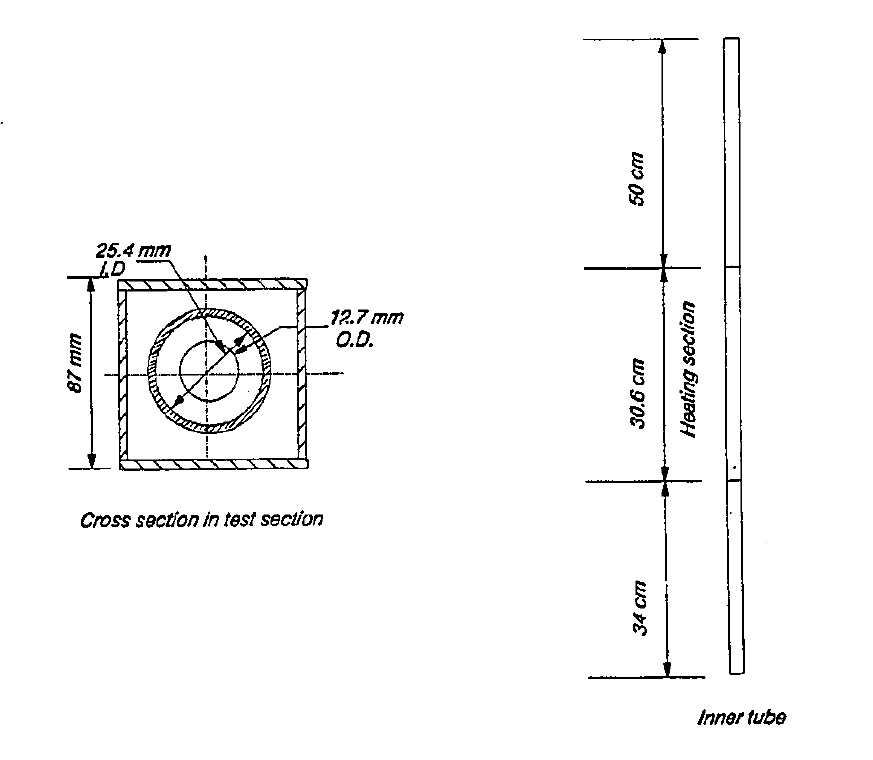
\includegraphics[width=.4\linewidth]{./03_benchmark/obrazky/zeitoun_geometrie.png}
%		\caption{Geometrie testovací trubice \cite{zeitoun1994subcooled}.}
%		\label{fig:zeitoun_geometrie}
%	\end{minipage}%
%	\begin{minipage}{.5\textwidth}
%		\centering
%		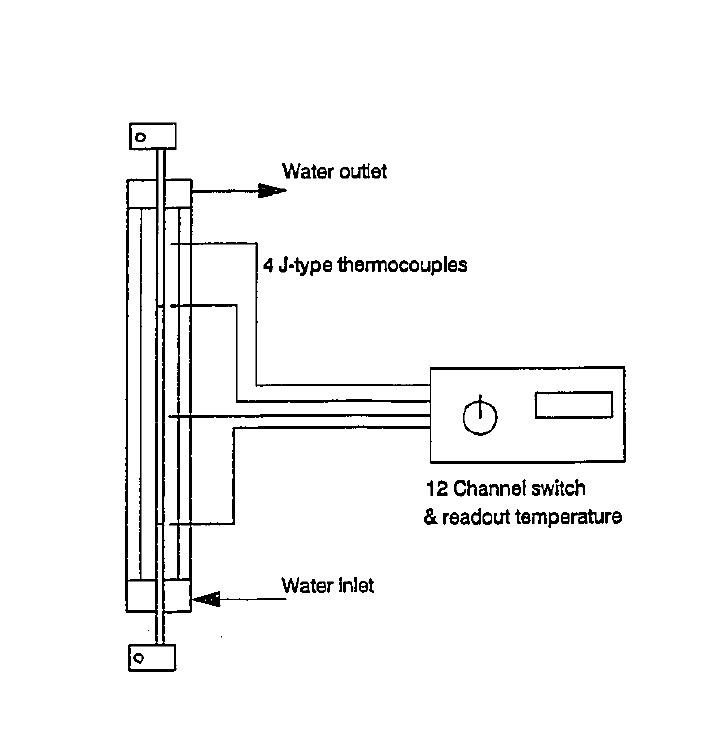
\includegraphics[width=.4\linewidth]{./03_benchmark/obrazky/zeitoun_circuit.png}
%		\caption{Testovací smyčka \cite{zeitoun1994subcooled}.}
%		\label{fig:zeitoun_circuit}
%	\end{minipage}
%\end{figure}
\begin{figure}
	\centering
	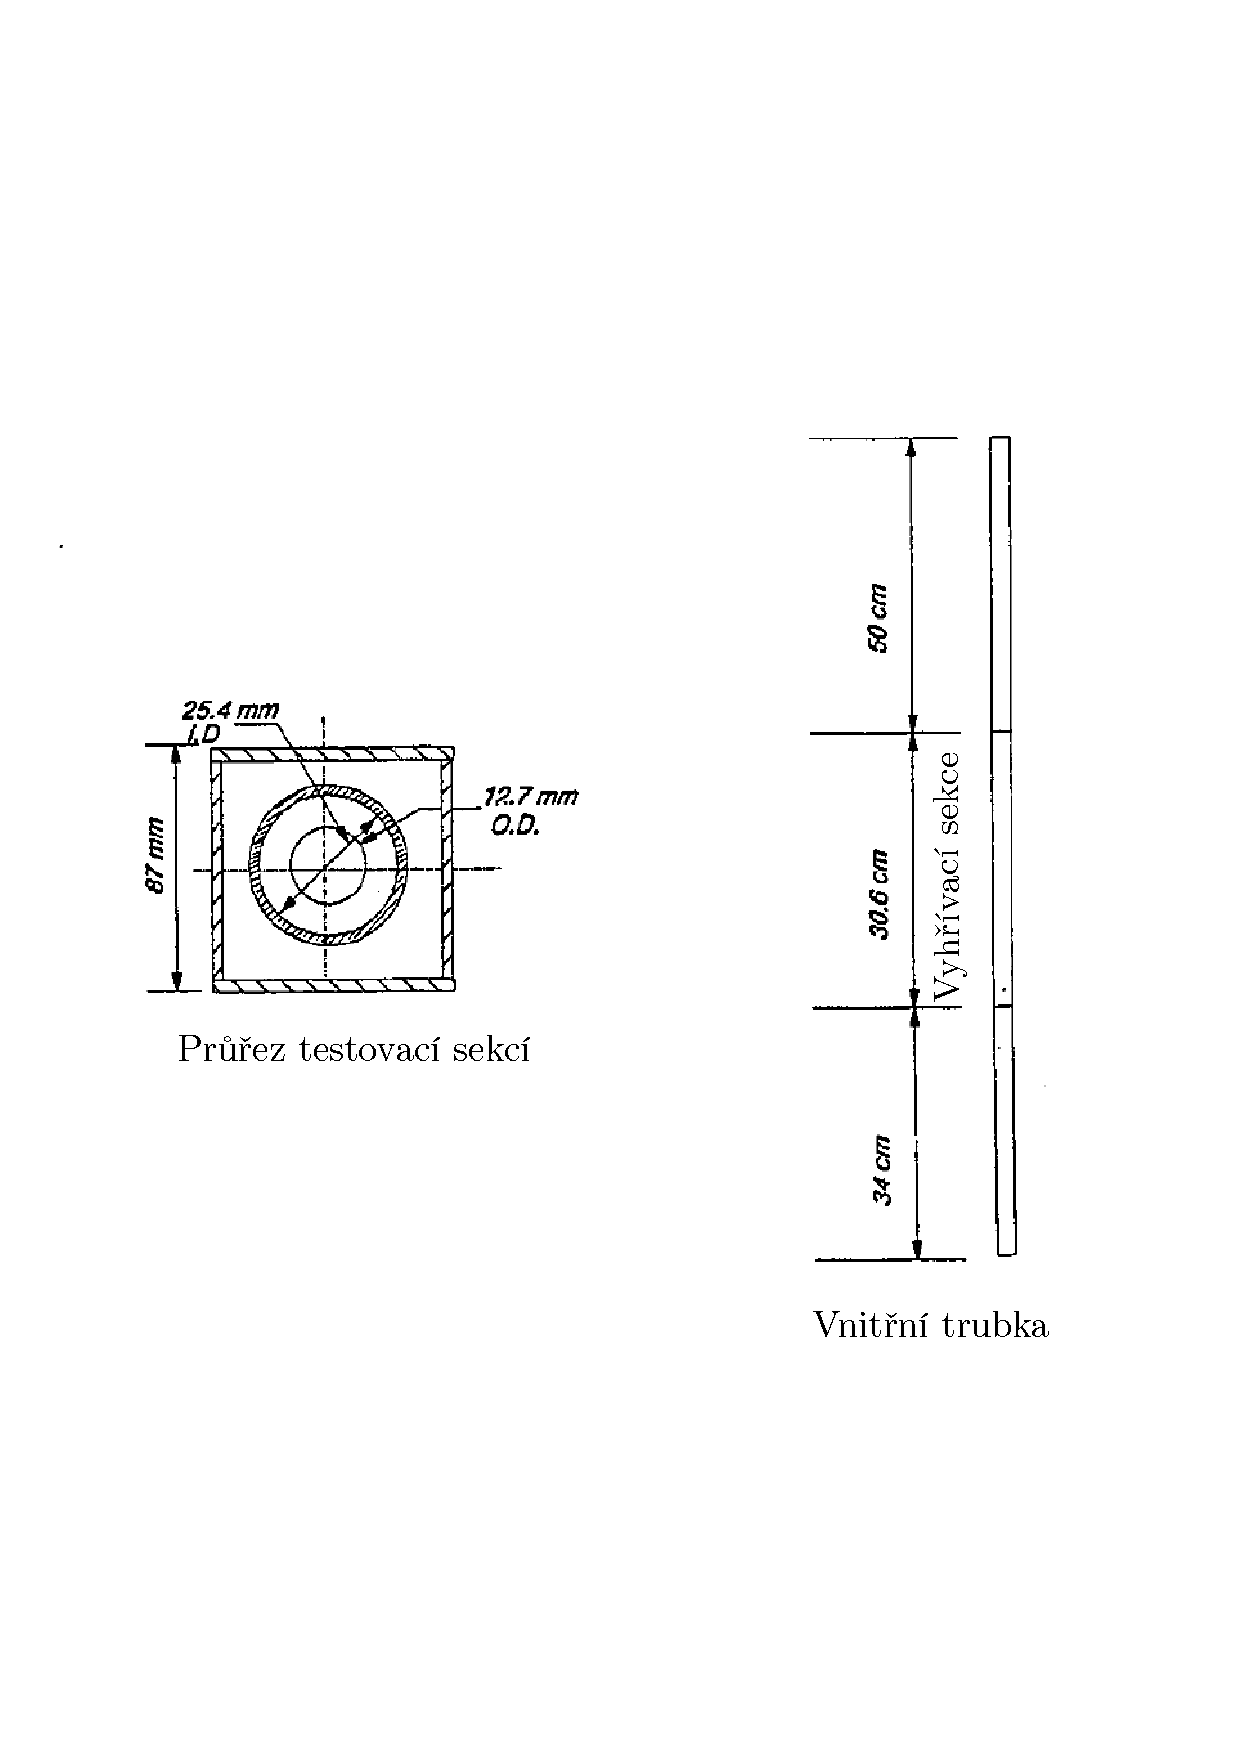
\includegraphics[width=0.8\textwidth, trim={0cm 8cm 0cm 8cm}, clip]{./03_benchmark/obrazky/zeitoun_geometrie_translated.pdf}
	\caption{Geometrie testovací trubice \cite{zeitoun1994subcooled}.}
	\label{fig:zeitoun_geometrie}
\end{figure}

\begin{figure}
	\centering
	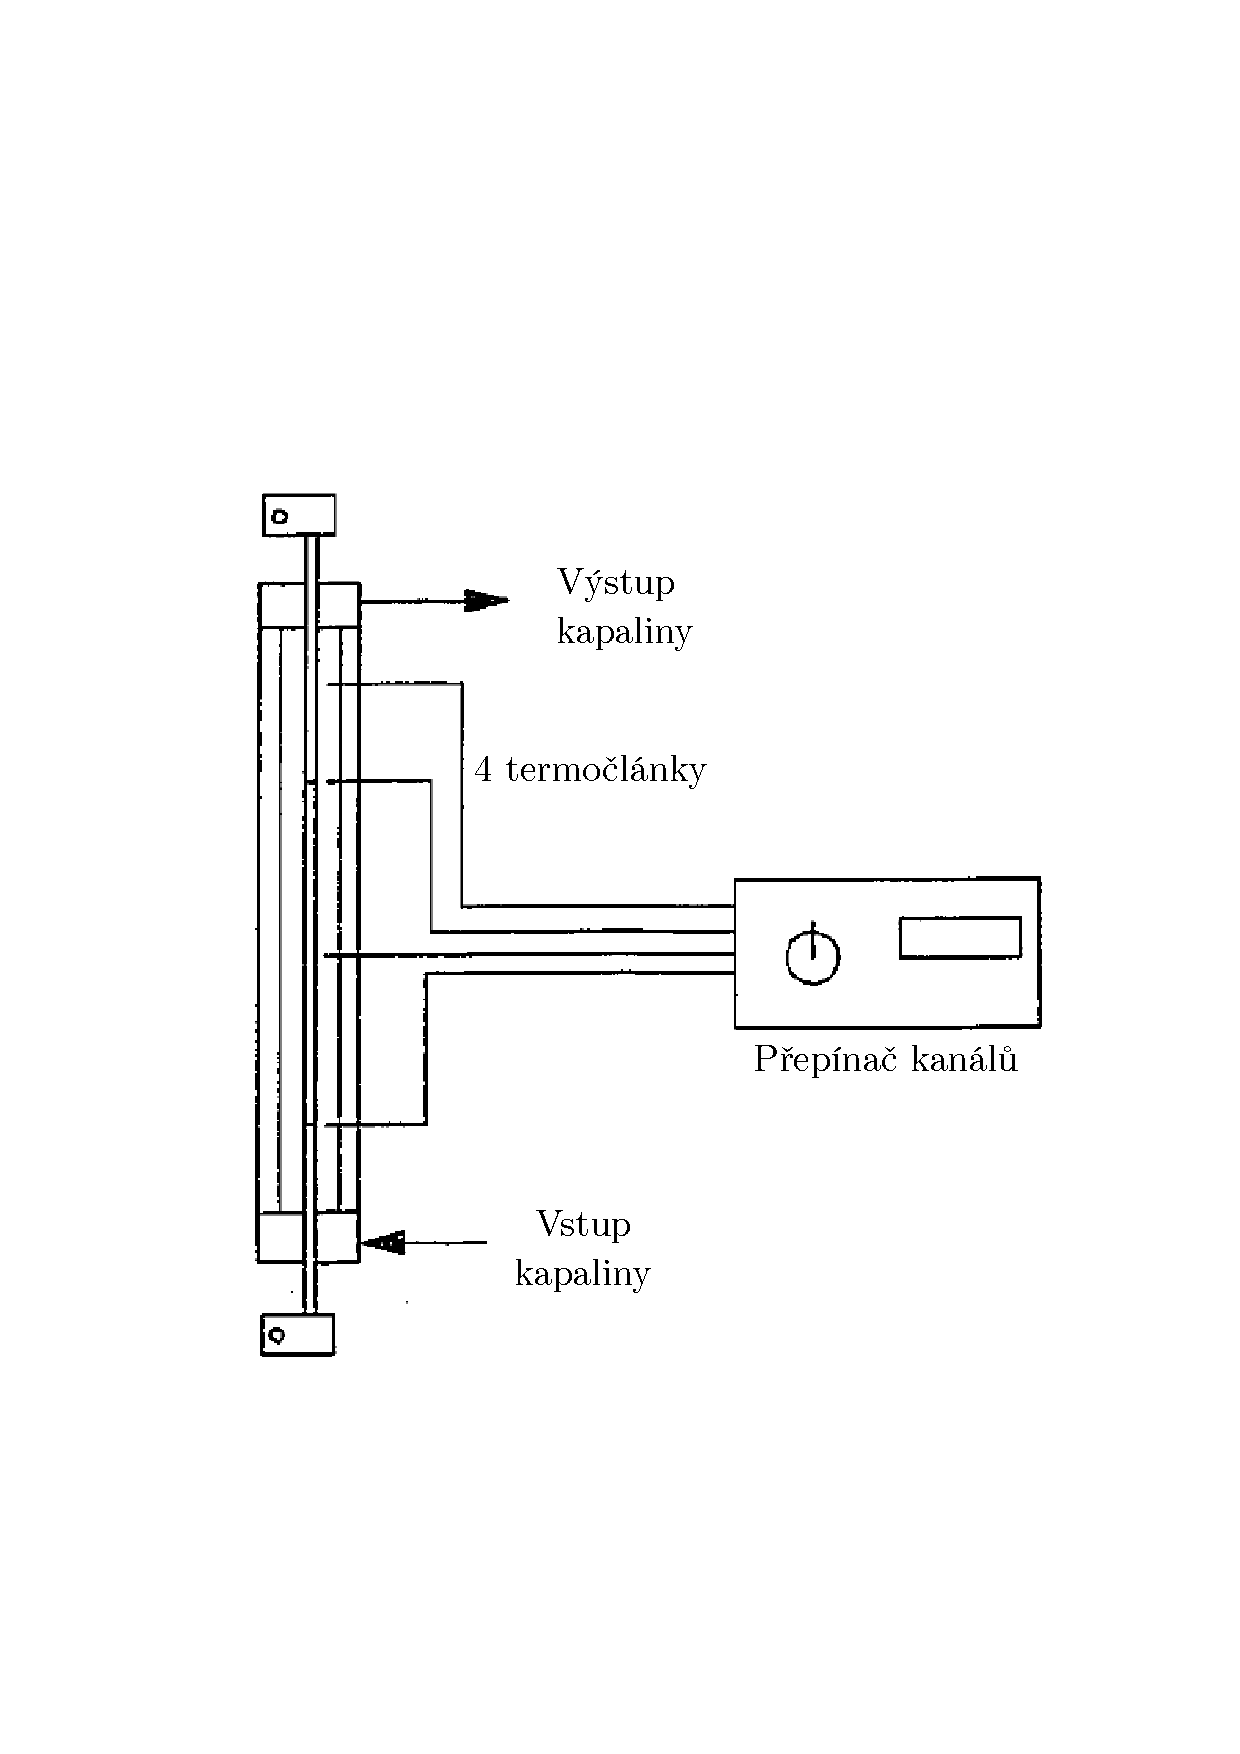
\includegraphics[width=0.8\textwidth, trim={0cm 5cm 0cm 8cm }, clip]{./03_benchmark/obrazky/zeitoun_circuit_translated.pdf}
	\caption{{Testovací smyčka \cite{zeitoun1994subcooled}.}}
	\label{fig:zeitoun_circuit}
\end{figure}


Během experimentu byly rovněž použity vysokorychlostní kamery, které pořizovaly snímky procesů varu a kondenzace uvnitř kanálu. To umožnilo podrobnější analýzu příslušných mechanismů přenosu tepla, jako například průběh dutinového koeficientu.
\section{Základní hydraulické komponenty v kódu RELAP5}
Vzhledem k tomu, že systémový kód RELAP5 využívá konstitutivní rovnice vycházející z teorie podobnosti, tak je uživatel nucen daný problém popsat pomocí přednastavených komponent. Dalším důvodem, proč je těchto komponent využíváno je usnadněná konvergence, která ovšem nemusí být pro komplexní modely nikdy zcela zajištěna. Program RELAP5 obsahuje celkem 17 typů komponent, avšak v této práci bude využito následujících 5 (Obr. \ref{fig:components_relap}). 
\begin{enumerate}
	\item Komponenta 1 - Kontrolní objemy představují konečnou oblast kapalinového systému, například potrubí nebo nádrž, v níž se předpokládají rovnoměrné vlastnosti kapaliny. Pro popis těchto vlastností jsou aplikovány jednorozměrné rovnice proudění.
	\item Komponenta 2 - Trubky slouží k přepravě kapalin z jednoho místa v systému na druhé. V kódu RELAP5 jsou potrubí reprezentována jako řada řídicích. Průtok kapaliny, tlakové ztráty a přenos tepla v potrubí se počítají pomocí jednorozměrných rovnic proudění.
	\item Komponenta 3 - Spojovací jednotky slouží k propojení dvou libovolných komponent. Jsou tvořeny kontrolním objemem, přičemž jsou zde aplikovány rovnice hmotnostní a energetické bilance.
	\item Komponenta 4 - Spojovací jednotky umožňují propojit i více komponent, které mají např. omezené množství výstupních cest. Plní funkci spojovací jednotky pro více komponent.
	\item Komponenta 5 - Objem/zdroj kapaliny sloužící ke stanovení okrajových podmínek (TDV).
	
\end{enumerate}  


Dále jsou v této práci využity tepelné jednotky (Heat structures) představující zdroj tepla. Přenos je popisován jednorozměrnými rovnicemi pro kondukci, konvekci a radiaci pro válcový, deskový či kulový zdroj. V této práci byly využity zdroje pouze válcové popsané výškou a vnějším a vnitřním průměrem \cite{relap_manual}.
\begin{figure}[H]
	\centering
	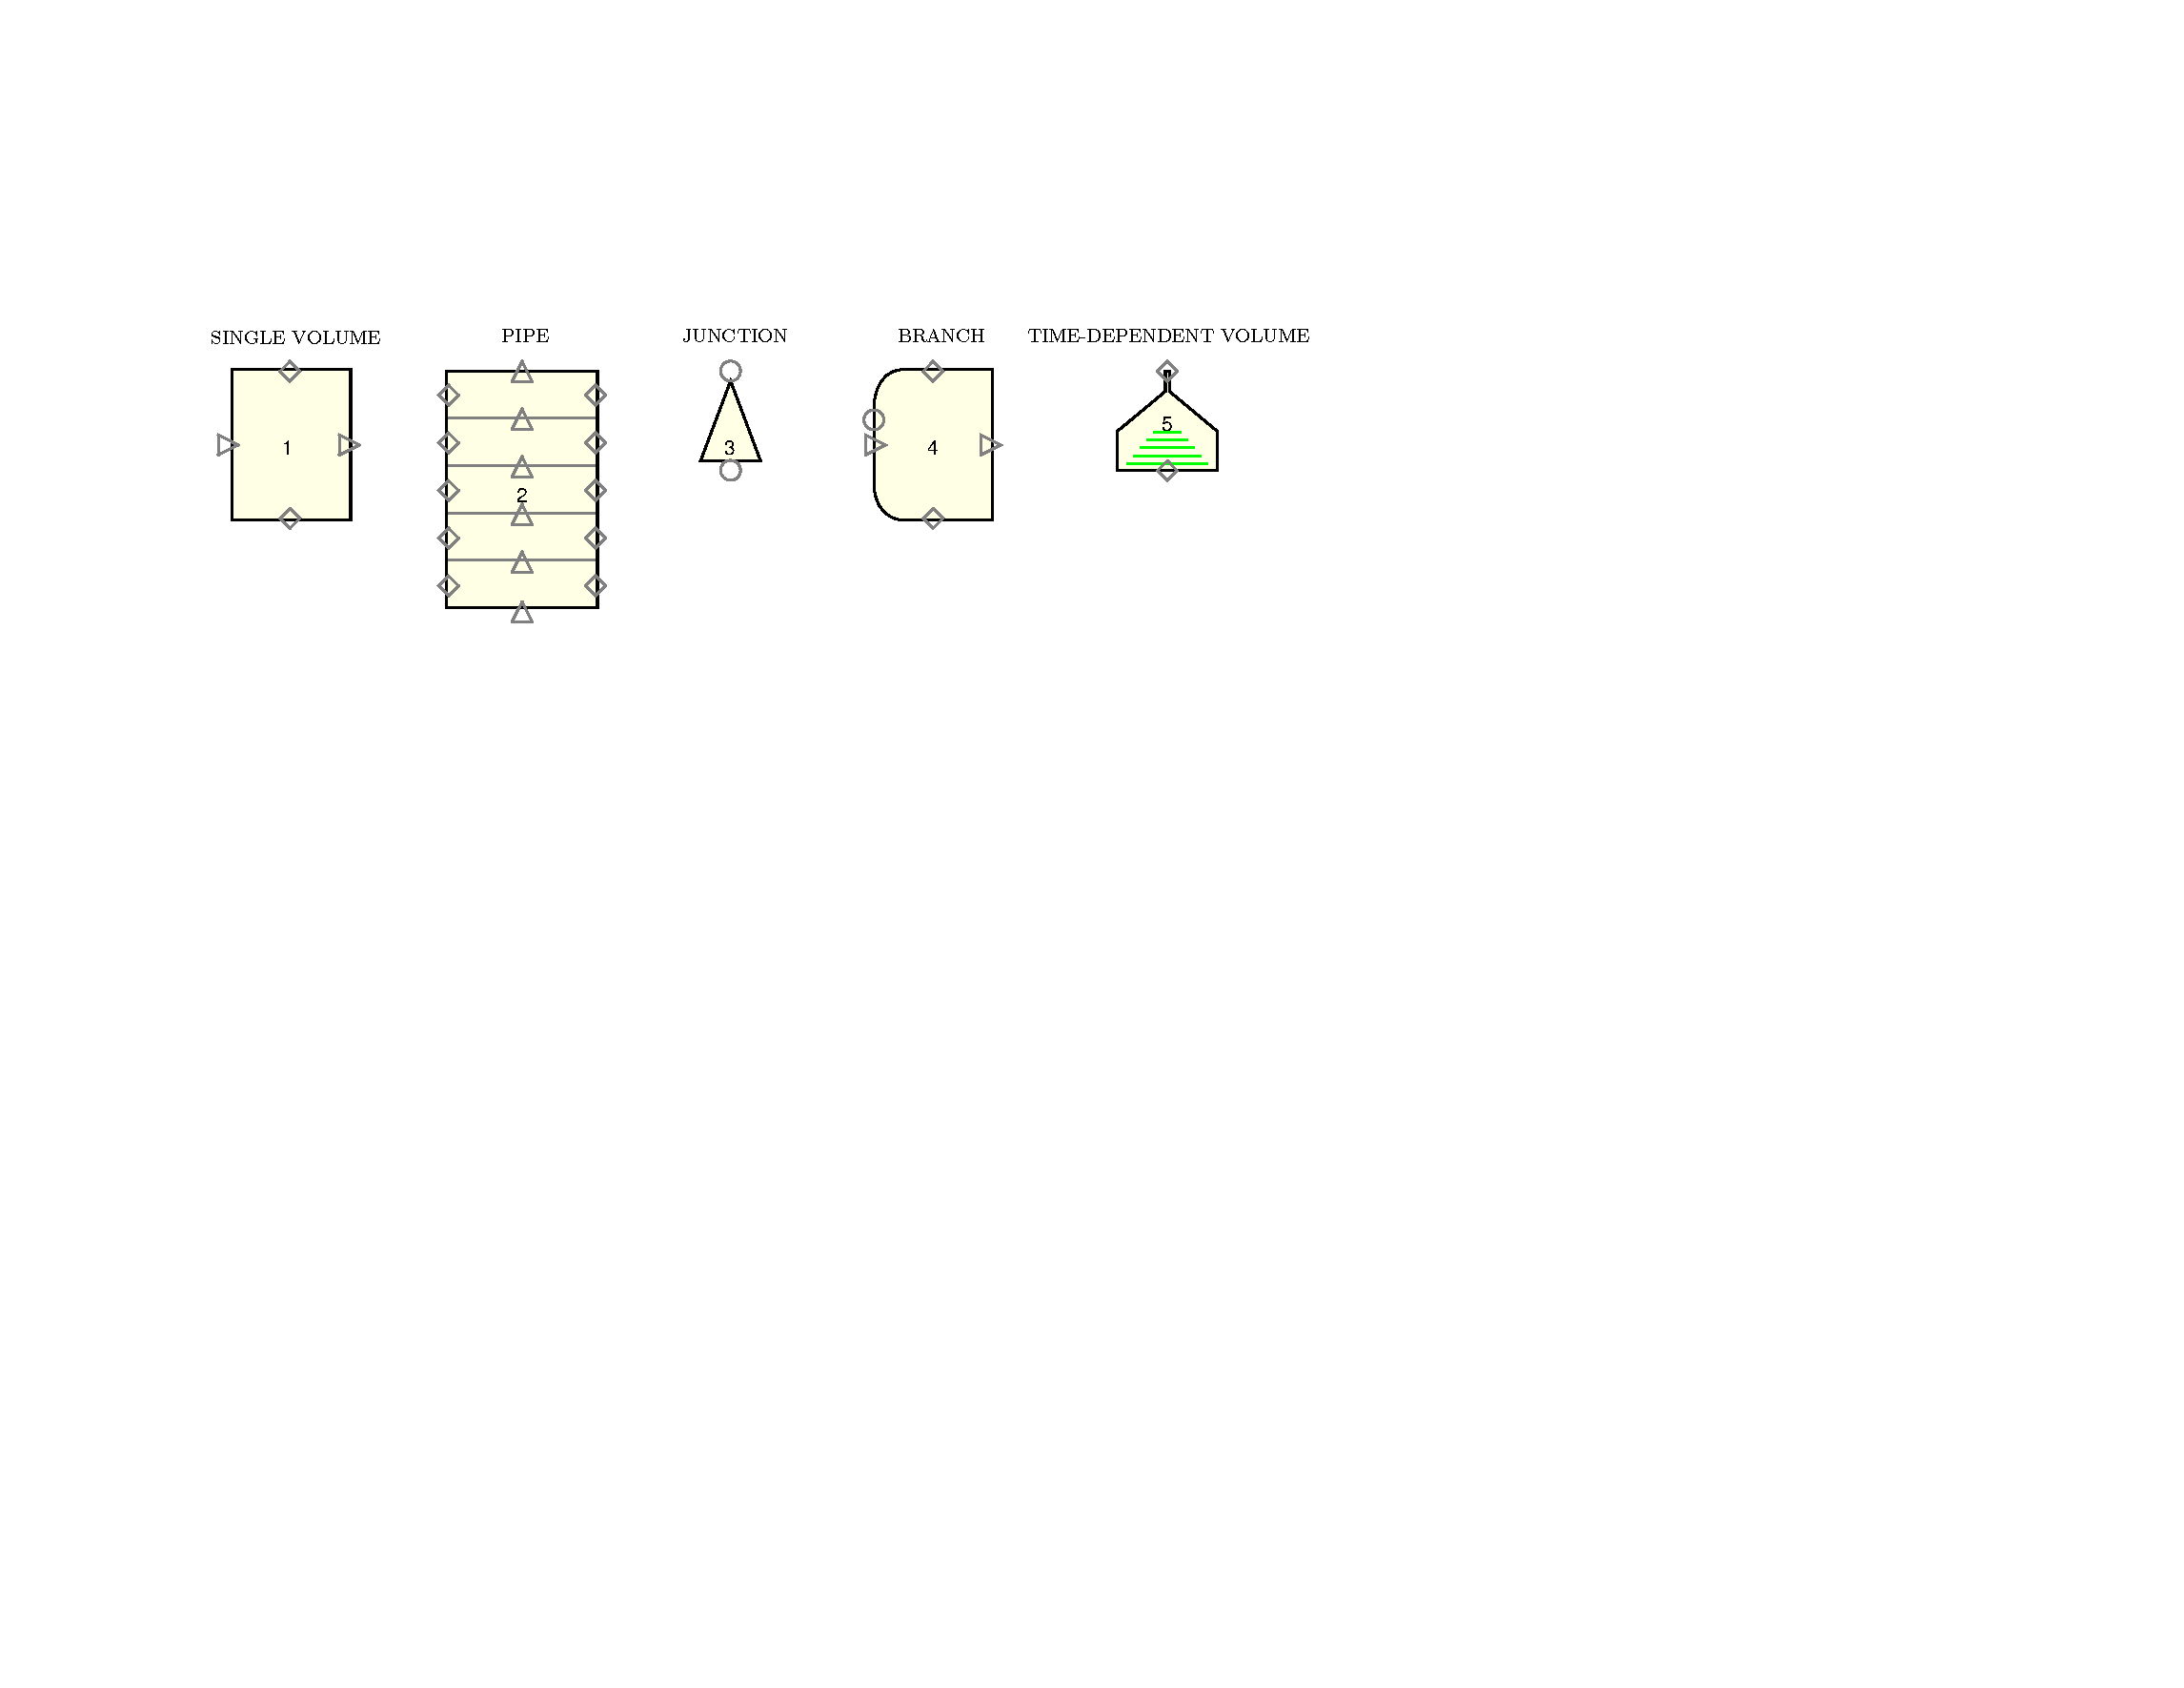
\includegraphics[clip, trim = 2cm 18cm 10cm 5cm, width=1.2\textwidth]{./03_benchmark/obrazky/HydraulicComponentsRELAPFinal.pdf}
	\caption{Hydraulické komponenty v programu RELAP5.}
	\label{fig:components_relap}
\end{figure}
Problematická se může jevit především nodalizace jednotlivých komponent a struktur. Využitím jemnějšího rozdělení je možné dosáhnout podrobnějšího popisu, avšak příliš jemná nodalizace může způsobit nestabilní výpočet a fyzikálně neodpovídající výsledky. Důvody proč příliš jemná nodalizace může být problematická jsou dva \cite{petruzzi2008thermal}:
\begin{itemize}
	\item velká část empirických vztahů zahrnutých do programu je získána z výpočtu s pevně danou nodalizací, což již z principu vede k rozdílným podmínkám,
	\item numerické simulace využívané v systémových kódech využívají uměle vloženou viskozitu za účelem získání stabilních výsledků.
\end{itemize}
Důležitým aspektem při popisu komplexního problému je propojení jednotlivých součástek, které může mít značný vliv na výsledné proudění. Pro nevhodně strukturovaných propojeních může docházet např. k různým obtokům, protiproudům či cirkulacím. Systémové kódy ve většině případů nabízejí model vytvořit z jednoduchých komponent, a proto je nutné při tvorbě modelu použít \uv{inženýrský odhad} a využít zkušenosti uživatele \cite{petruzzi2008thermal}. 

\section{Model v RELAP5}
Cílem této sekce je představit zjednodušený model experimentální sestavy popsané v \cite{zeitoun1994subcooled}.

Pro jednoduchost byly podmínky v testovací sekci experimentální smyčky simulovány rozdílem v tlaku na vstupu a výstupu trubky, konstantním objemovým, výkonem elektrického ohříváku a vstupní, resp. výstupní teplotou vody.  

 Vytvořený model je vyobrazen na Obr. \ref{fig:zeitoun_model},  modelované podmínky vycházející z \cite{zeitoun1994subcooled} jsou uvedeny v Tab. \ref{tab:zeitoun_podminky}. Tlak a teplota na vstupu byly nastaveny pomocí časově závislé objemové komponenty 1 (dále TDV), průtok byl nastaven časově závislou spojovací jednotkou 2 (dále TDJ) a tlak na výstupu komponentou TDV 9. Jelikož geometrie trubek je v programu RELAP5 značně omezená, k aproximaci průtočné trubky byla využita kruhová trubka s odpovídajícím hydraulickým průměrem $ d_h = 0,0127 $ m. Geometrie testovací trubice je vykreslena na Obr. \ref{fig:zeitoun_geometrie}. Průtočná plocha má tvar mezikruží s vnějším průměrem 25,4 mm a el. ohřívák tvar válce s průměrem 12,7 mm.
 \begin{figure}[h]
	\centering
	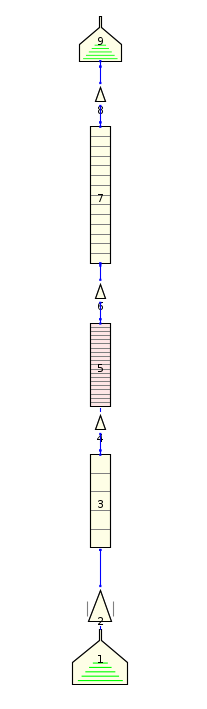
\includegraphics[width=0.3\textwidth]{./03_benchmark/obrazky/zeitoun_model.png}
	\caption{Termohydraulický model testovací trubice - RELAP.}
	\label{fig:zeitoun_model}
\end{figure}
\begin{table}[h]
	\centering
	\caption{Podmínky pro ověření modelu \cite{zeitoun1994subcooled}.}
	\label{tab:zeitoun_podminky}
	\begin{tabular}{cccccc}
		\hline
	experiment & P (W)            & G (kg/m$^2$s) & p$_{\text{in}}$ (kPa) & T$_{\text{in}}$ (K) & p$_{\text{out}}$ (kPa) \\
	\hline \hline
	BC1        & 2607 & 161,2      & 114         & 363,75    & 103,15    \\
	BC7        & 5869 & 208,05     & 114         & 356,65    & 103,15    \\
	BC9        & 5925 & 485,34     & 132         & 361,85    & 121,14   \\
	BC13       & 7366 & 348,94     & 137         & 361,15    & 126,13     \\ \hline
		\end{tabular}

	
\end{table}
\section{Výsledky experimentů a výpočtů}
Na Obr. \ref{fig:zeitoun_bc1}, \ref{fig:zeitoun_bc7}, \ref{fig:zeitoun_bc9} a \ref{fig:zeitoun_bc13} jsou vykresleny průběhy dutinového koeficientu v vyhřívané sekci testovací trubice. Ve všech případech je možné rozdělit oblasti na silně podchlazenou oblast (\uv{Highly subcooled region}) a slabě podchlazenou oblast (\uv{Low subcooling region}). Přechod mezi těmito regiony je nazýván \uv{Onset of significant void} a ve všech případech je situován ve výšce okolo 0,2 m \cite{KONCAR2003255}.  

Z Obr. \ref{fig:zeitoun_bc1}, \ref{fig:zeitoun_bc7}, \ref{fig:zeitoun_bc9} a \ref{fig:zeitoun_bc13} je jasně vidět, že zatímco ve vysoce podchlazené oblasti je dutinový koeficient menší ve srovnání s experimenty, tak v slabě podchlazené oblasti dává program RELAP5 nadhodnocené výsledky. Kvalitativně jsou ovšem výsledky ve shodě s měřením. Ve všech případech je přechod mezi výše zmíněnými oblastmi v okolí bodu 0,2 m, kdy dochází k výraznému nárůstu dutinového koeficientu. Důvodem nesrovnalostí může být jak jednak zjednodušený popis experimentální smyčky, tak extrapolace empirických vztahů odvozených pro vysoké tlaky. 

Při porovnání dutinového koeficientu vycházejícího z modelu \ref{fig:zeitoun_model} a výsledků z \cite{KONCAR2003255} lze pozorovat obdobné odchylky od experimentálních dat. Přestože se jedná o rozdílný model a rozdílnou verzi programu RELAP5, tak lze vytvořený model považovat za dostatečně přesný. 

\begin{figure}[p]
	\centering
	\begin{minipage}{.5\textwidth}
		\centering
		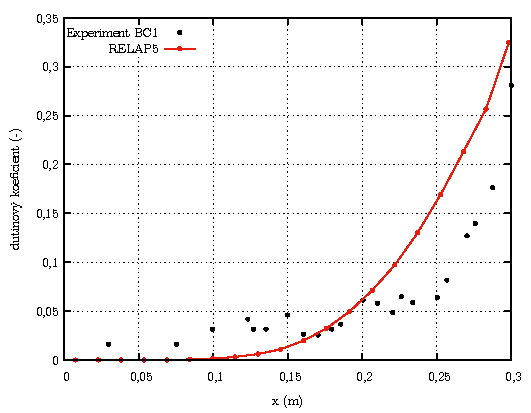
\includegraphics[width=\linewidth]{./03_benchmark/grafy/srovnani_exp1.pdf}
		\caption{Srovnání dutinového koeficientu - exp. BC1.}
		\label{fig:zeitoun_bc1}
	\end{minipage}%
	\begin{minipage}{.5\textwidth}
		\centering
		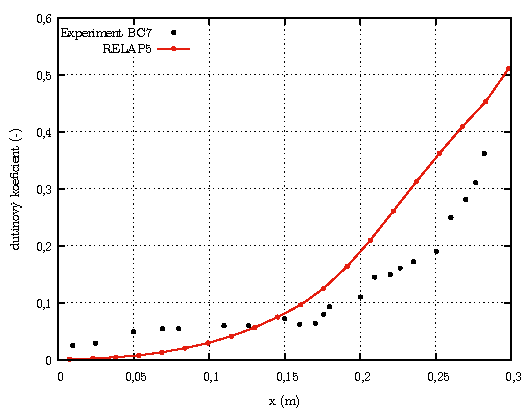
\includegraphics[width=\linewidth]{./03_benchmark/grafy/srovnani_exp2.pdf}
		\caption{Srovnání dutinového koeficientu - exp. BC7.}
		\label{fig:zeitoun_bc7}
	\end{minipage}
\end{figure}

\begin{figure}[p]
	\centering
	\begin{minipage}{.5\textwidth}
		\centering
		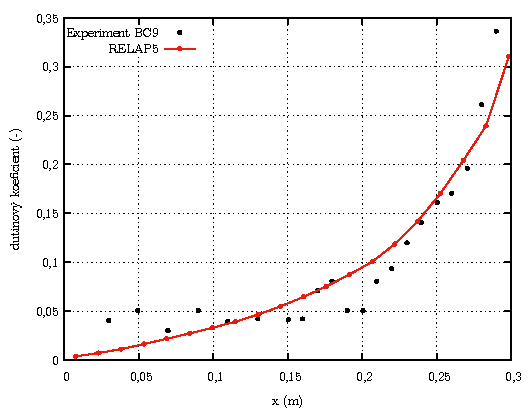
\includegraphics[width=\linewidth]{./03_benchmark/grafy/srovnani_exp3.pdf}
		\caption{Srovnání dutinového koeficientu - exp. BC9.}
		\label{fig:zeitoun_bc9}
	\end{minipage}%
	\begin{minipage}{.5\textwidth}
		\centering
		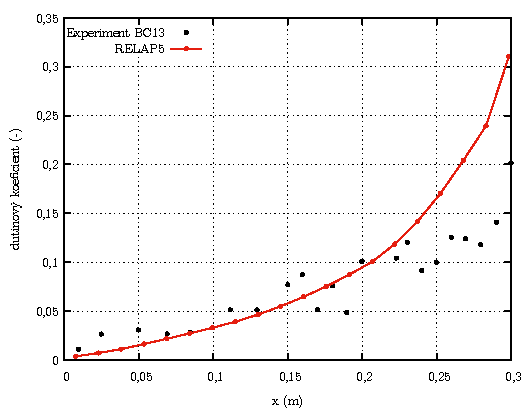
\includegraphics[width=\linewidth]{./03_benchmark/grafy/srovnani_exp4.pdf}
		\caption{Srovnání dutinového koeficientu - exp. BC13.}
		\label{fig:zeitoun_bc13}
	\end{minipage}
\end{figure}